\documentclass[12pt, a4paper]{article}
\usepackage[margin=25.4mm]{geometry}
\usepackage{charter} % Font
\usepackage{graphicx} % Required for inserting images
\usepackage{amsmath}
\usepackage{amsfonts}
\usepackage{amssymb}
\usepackage{hyperref} % Links
\usepackage[]{parskip} % Paragraph indentation and margins
\usepackage{subcaption}

\usepackage[english]{babel}
\usepackage[T1]{fontenc}

\usepackage[backend=biber, style=numeric, sorting=none]{biblatex}
\usepackage{csquotes}

%------ Metadata ------%
\hypersetup{
    pdftitle={AI Lab LoL Report},
    pdfauthor={Nicolas Jurquet},
    pdfsubject={Ecamania Esports Project},
    pdfkeywords={AI, LoL, Esport, ML},
    colorlinks=true,
    linkcolor=black,
    urlcolor=blue,
    citecolor=blue
}

\renewcommand\labelitemi{---} % Change itemize bullet style to dashes


\begin{document}
\begin{titlepage}
    \begin{center}
        \vspace*{1cm}
        
\includegraphics[width=0.6\textwidth]{figures/ECAM_logo.jpg}\\
        
        \vspace{3cm}

        \setlength{\parskip}{0pt}
        \hrule
        \vspace{0.5cm}
        \huge
        \textsc{\textbf{Ecamania Esports Project\\Report}}\\
        \vspace{0.5cm}
        \hrule
        
        \vspace{1cm}
        
        \LARGE
        \textsc{AI Lab}\\

        \vspace{2cm}

        \large
        \setlength{\tabcolsep}{10pt}
        \renewcommand{\arraystretch}{1.5}
        \begin{tabular}{ccc}
            \textbf{First Name :} & \textbf{Last Name :} & \textbf{Matricule :} \\
            Jurquet & Nicolas & 21211
        \end{tabular}

        \vfill
        
        \textbf{Haute École ICHEC - ECAM - ISFSC}\\
        \medskip

        % Automate academic years
        \newcommand{\yearOne}{
            \the\numexpr \the\year - \ifnum\month<9 1\else 0\fi\relax
        }
        \newcommand{\yearTwo}{
            \the\numexpr \the\year + \ifnum\month<9 0\else 1\fi\relax
        }
        Academic year \yearOne\space --\yearTwo
    \end{center}
\end{titlepage}


\section{Introduction}
\textbf{Ecamania Esports Project} is a project that aims to find the best \emph{League of Legends (LoL)} team to recruit for the ECAM team.
It is asked to analyse a dataset of LoL games by training Machine Learning (ML) and Deep Learning (DL) models to:
\begin{itemize}
    \item Determine, based on in-game statistics of a single player, whether their team won or lost the match.
    \item Identify the most important quantifiable variables that players should focus on to increase their chances of winning.
    \item Determine the most talented players Ecamania could recruit for the next season.
\end{itemize}

Considering the lack of time and setup problems I had, only the first point was completed and analysis/explainations were not developped as much as intended.

The methodology adopted was to first visualize and understand the dataset, then see which features could be relevant to predict the outcome of a game or its interaction with other features, a preprocessing step was then used, and finally models were trained and evaluated to predict the outcome of a game.

All the code created during the project is available on my \href{https://github.com/NJurquet/neuralol}{GitHub repository}.

\section{Dataset visualization}
Upon displaying some of the first rows of the \texttt{game\_players\_stats.csv} file, \textbf{28} columns were identified and a total of \textbf{374554} rows of player games.
A total of \textbf{37459} unique games were played, with a total of \textbf{4953} players, and within \textbf{844} different teams.

\begin{table}[!ht]
    \centering
    \small % Reduced font size for the table
    \begin{tabular}{|c|c|c|}
        \hline
        \texttt{game\_id} & \texttt{player\_id} & \texttt{player\_name} \\
        \hline
        \texttt{team\_id} & \texttt{team\_name} & \texttt{team\_acronym} \\
        \hline
        \texttt{role} & \texttt{win} & \texttt{game\_length} \\
        \hline
        \texttt{champion\_name} & \texttt{team\_kills} & \texttt{tower\_kills} \\
        \hline
        \texttt{inhibitor\_kills} & \texttt{dragon\_kills} & \texttt{herald\_kills} \\
        \hline
        \texttt{baron\_kills} & \texttt{player\_kills} & \texttt{player\_deaths} \\
        \hline
        \texttt{player\_assists} & \texttt{total\_minions\_killed} & \texttt{gold\_earned} \\
        \hline
        \texttt{level} & \texttt{total\_damage\_dealt} & \texttt{total\_damage\_dealt\_to\_champions} \\
        \hline
        \texttt{total\_damage\_taken} & \texttt{wards\_placed} & \texttt{largest\_killing\_spree} \\
        \hline
        \texttt{largest\_multi\_kill} & & \\
        \hline
    \end{tabular}
    \caption{Dataset columns}
    \label{tab:dataset_columns}
\end{table}

\begin{figure}[!ht]
    \centering
    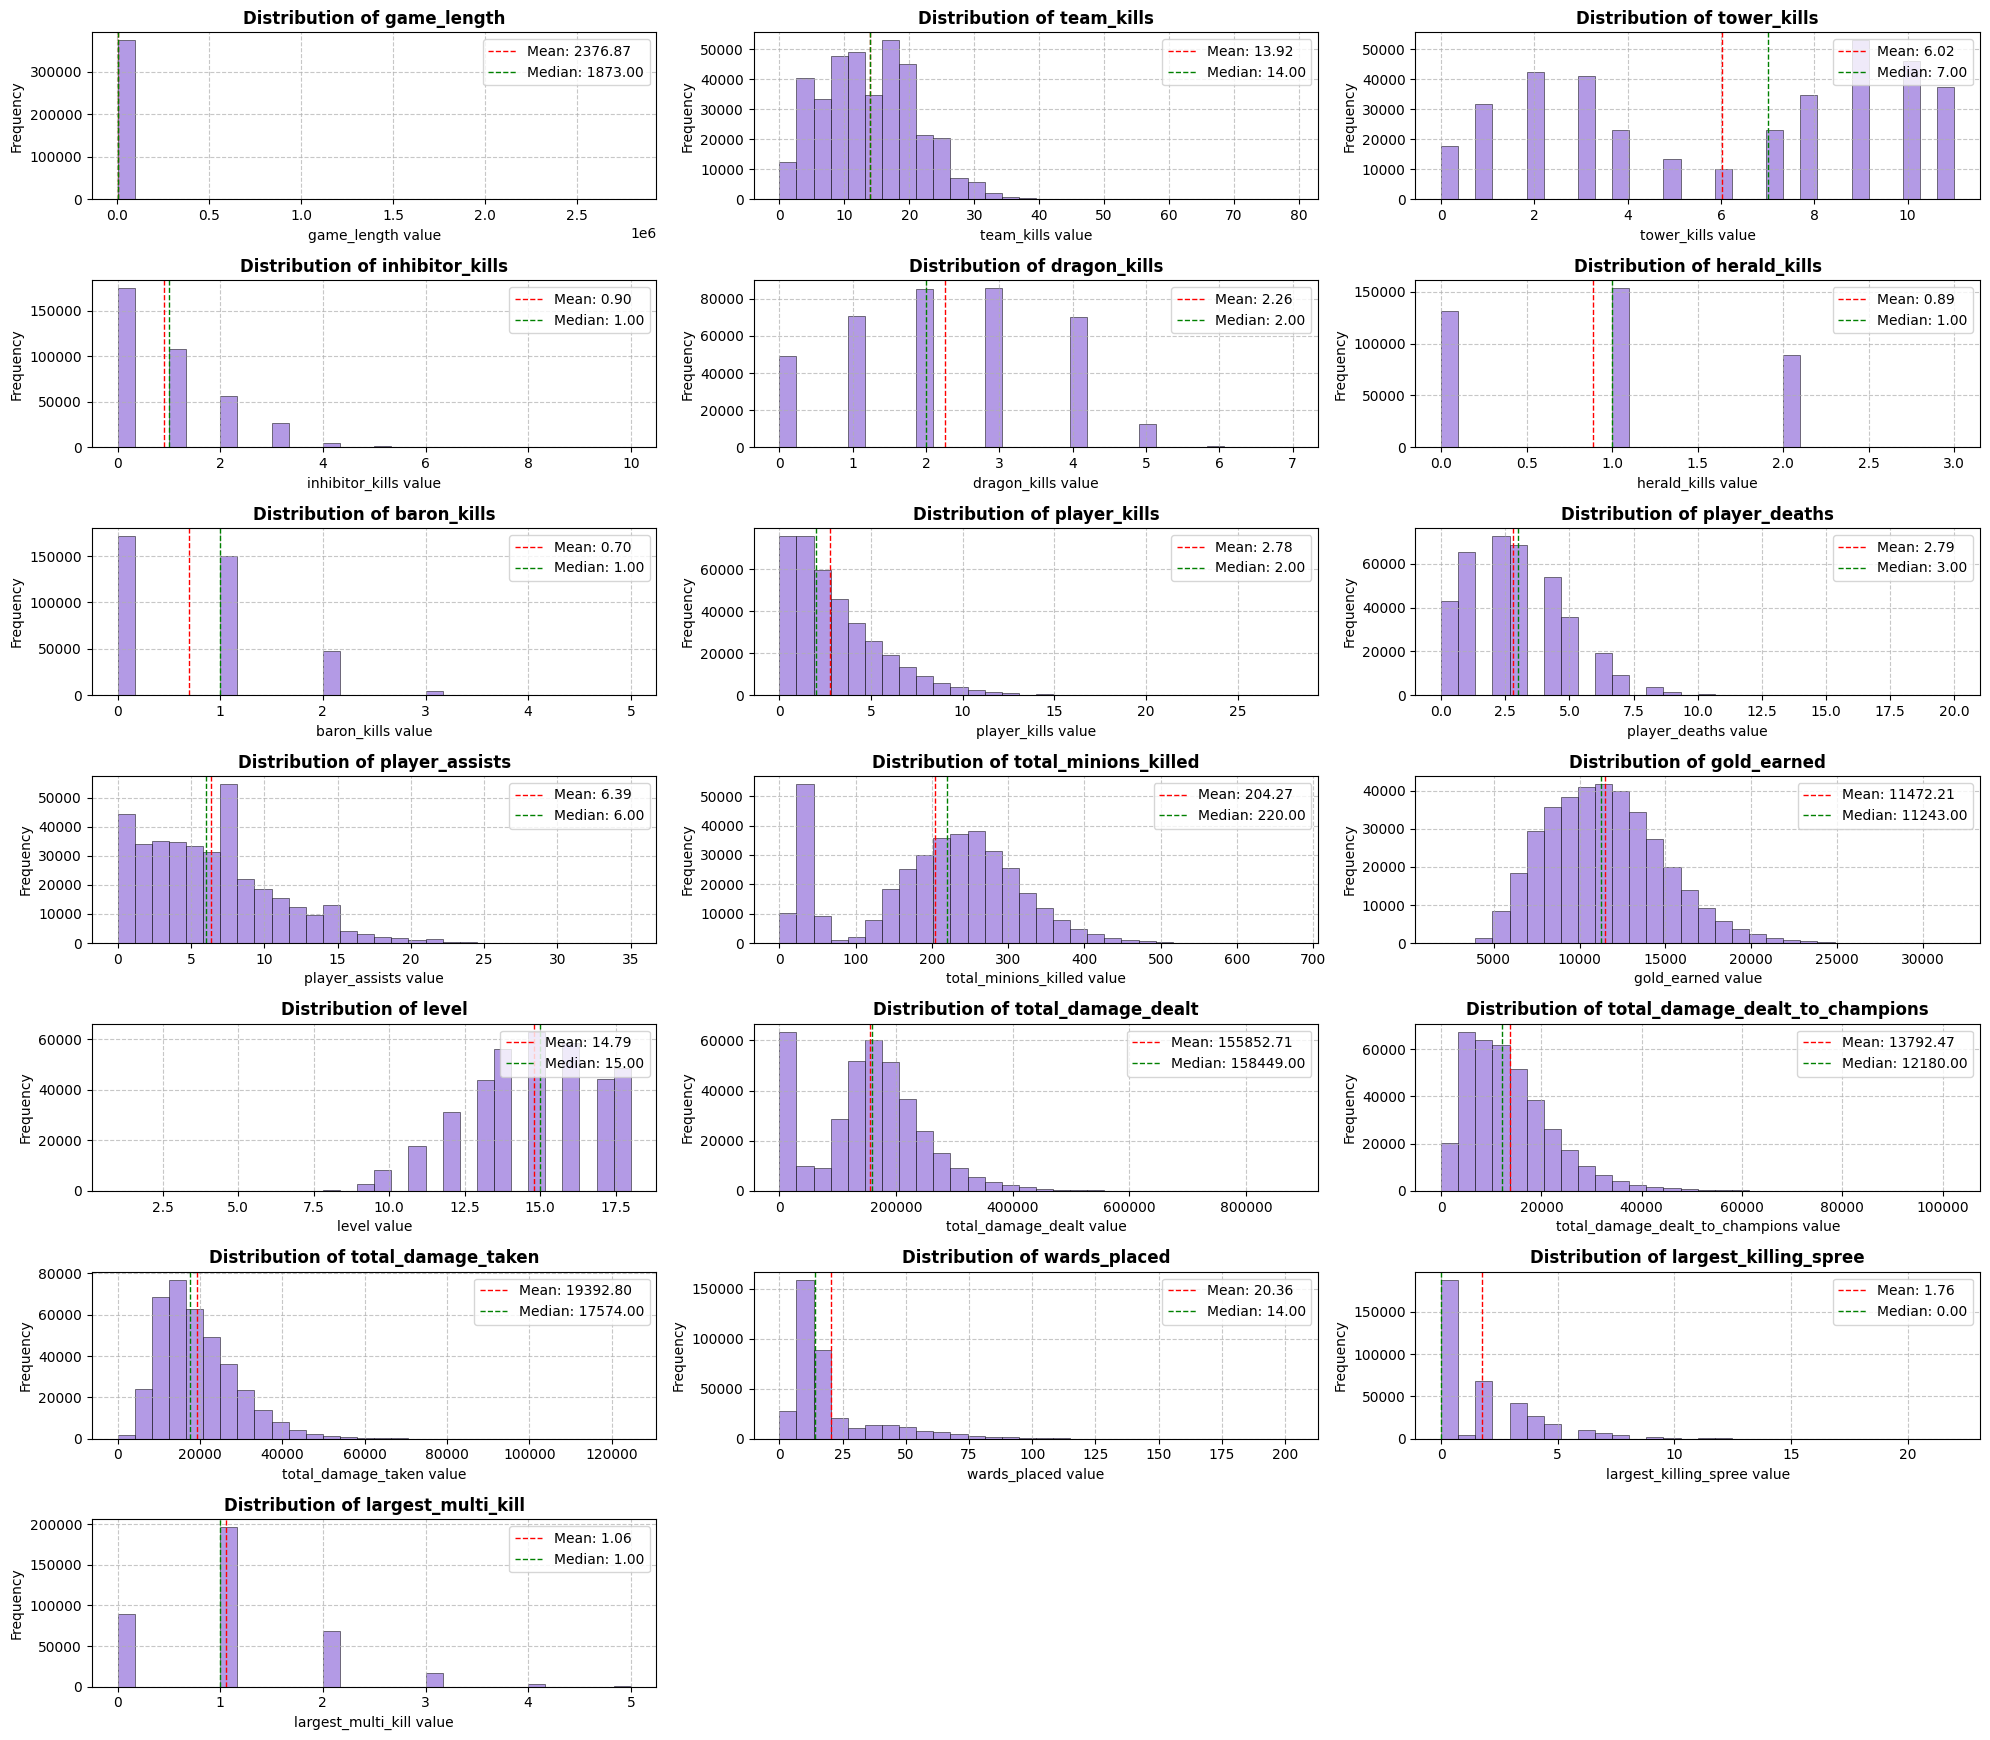
\includegraphics[width=0.7\textwidth]{figures/0_visualization_dataset_features.png}
    \caption{Distribution of all numerical features in the dataset}
    \label{fig:dataset_features_distribution}
\end{figure}

\figurename~\ref{fig:dataset_features_distribution} shows the distribution of all numerical features in the dataset.
It can directly be noted that the \texttt{game\_length} feature seems to have outliers as all the data is on the left side of the graph.
We also have the same problem with the number of wards placed in a match reaching values of 200 which seems to be very unlikely.
Limiting those values to a meaningful maximum value result in a better distribution of the data shown in \figurename~\ref{fig:game_length_wards_distribution}.

\begin{figure}[!ht]
    \centering
    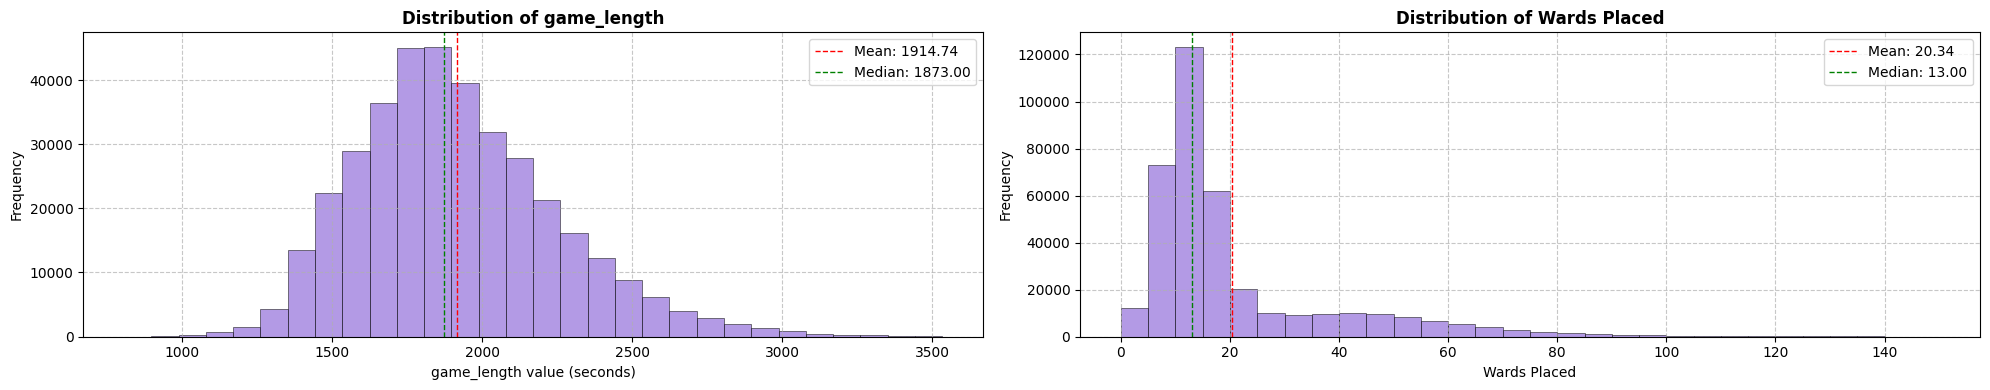
\includegraphics[width=0.8\textwidth]{figures/0_visualization_game_length_without_outliers.png}
    \caption{Distribution of game length and wards placed without outliers}
    \label{fig:game_length_wards_distribution}
\end{figure}

The dataset also contained some missing values but only for the \texttt{team\_acronym} column (0.077425\% of it) which does not impact plyers stats and performance.
Missing values will be addressed later in the preprocessing step.

An interesting statistic is the total number of games played and by each player represented on \figurename~\ref{fig:games_played}.

\begin{figure}[!ht]
    \centering
    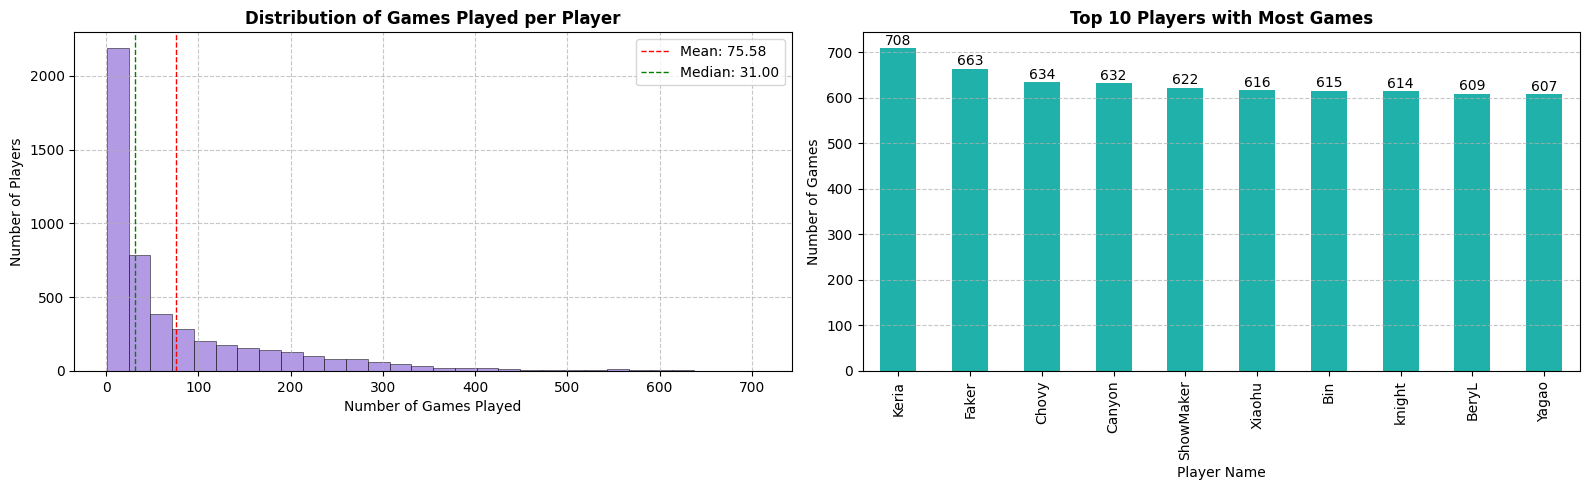
\includegraphics[width=0.8\textwidth]{figures/0_visualization_games_played.png}
    \caption{Total number of games played by each player}
    \label{fig:games_played}
\end{figure}
The tendency is showing that players considered as very good players are playing a lot of games, while there is a lot of players playing only a few games.
Filtering the dataset to only keep players with a minimum amount of games could be a good idea to avoid considering players that are probably not playing at a high level.

There is also 168 different champions played across the dataset, showed in \figurename~\ref{fig:champions_played} and \figurename~\ref{fig:champions_played_per_role}.

\begin{figure}[!ht]
    \centering
    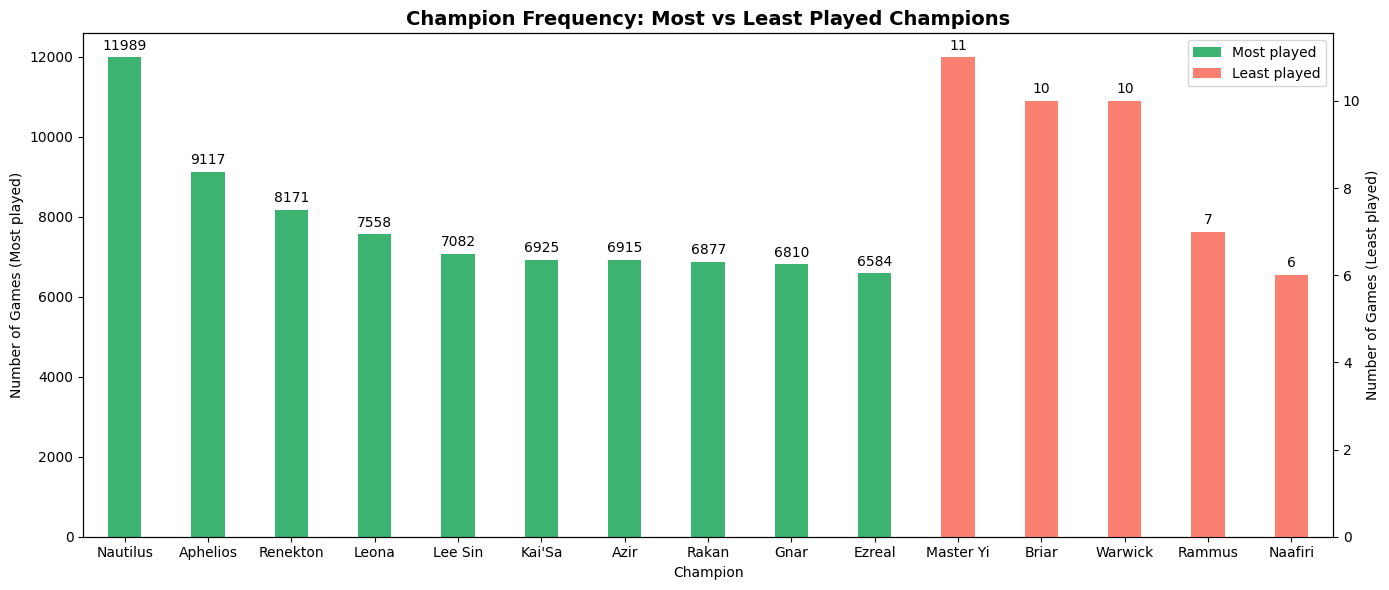
\includegraphics[width=0.8\textwidth]{figures/0_visualization_most_played_champs.png}
    \caption{Most vs. Least played champions}
    \label{fig:champions_played}
\end{figure}

\begin{figure}[!ht]
    \centering
    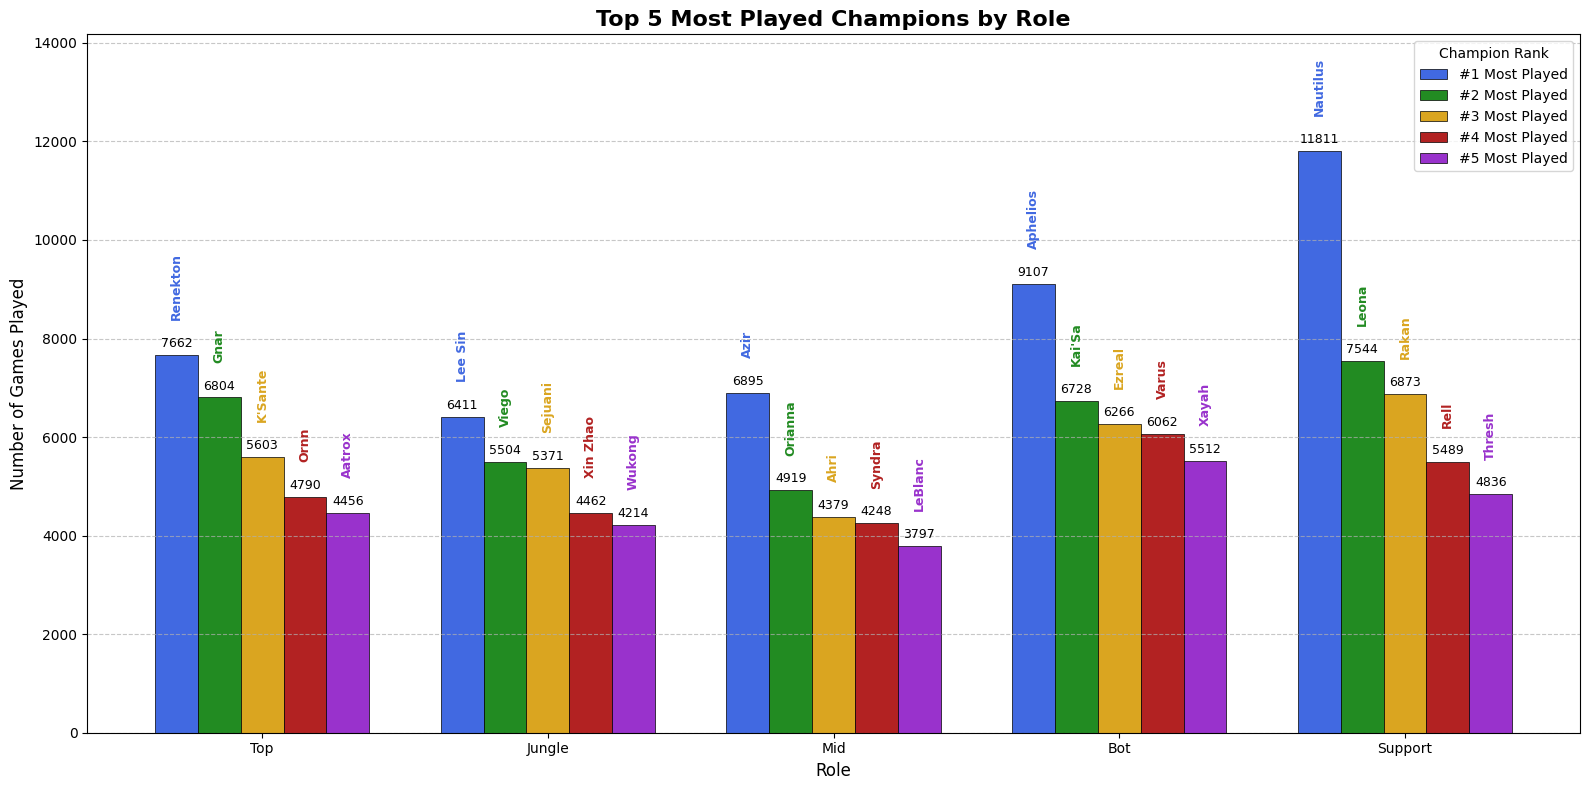
\includegraphics[width=0.8\textwidth]{figures/0_visualization_most_played_champs_by_role.png}
    \caption{Most played champions per role}
    \label{fig:champions_played_per_role}
\end{figure}

\section{Feature analysis}
To analyse the features and know which one are worth to be interested in, a Mutual Information (MI) graph was drawn.

\begin{figure}[!ht]
    \centering
    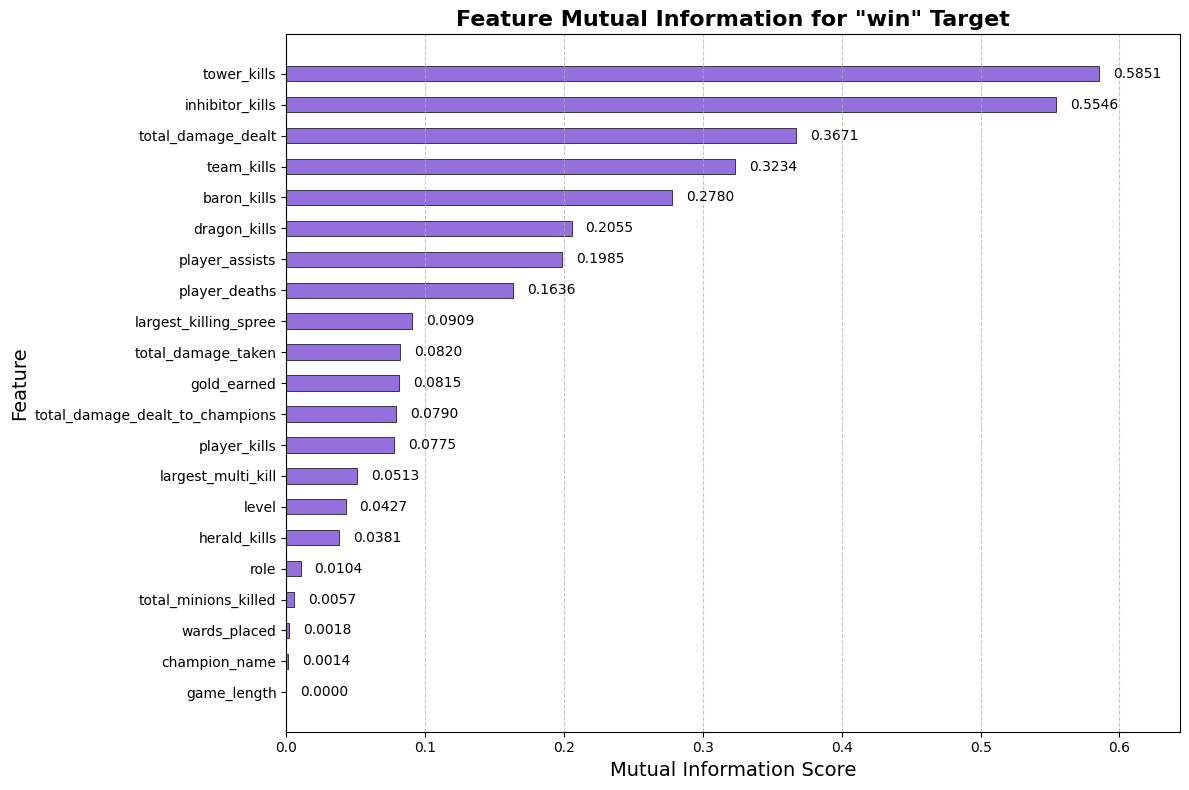
\includegraphics[width=0.8\textwidth]{figures/0_visualization_features_MI.png}
    \caption{Mutual Information scores for win target}
    \label{fig:mutual_information}
\end{figure}

A correletion heatmap was also used in \figurename~\ref{fig:correlation_heatmap} to also see the correlation between features.

\begin{figure}[!ht]
    \centering
    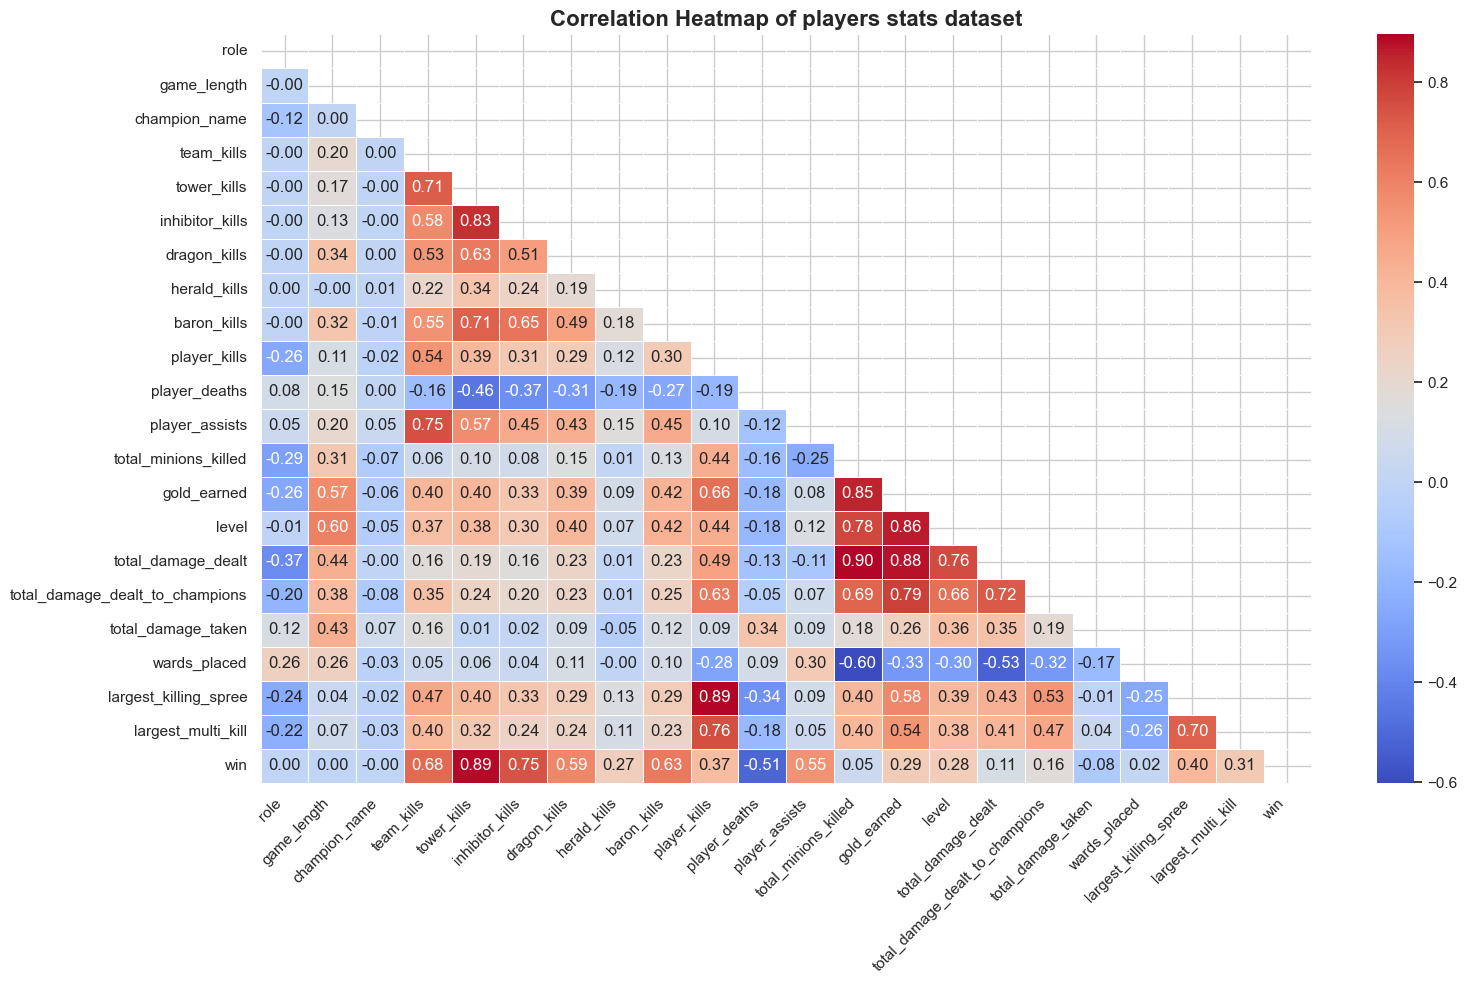
\includegraphics[width=0.9\textwidth]{figures/0_visualization_features_correlation.png}
    \caption{Correlation heatmap}
    \label{fig:correlation_heatmap}
\end{figure}

Some interesting features of MI scores were represented in histograms and available in \appendixname~\ref{sec:features_histogram}.

Some new features were also created based on their correlation and the LoL knowledge I have, to predict if a player won the match or not.
They are all represented in \appendixname~\ref{sec:new_features_histogram}.
It can clearly be seen that there is a distinction between winning and loosing based on the value of these features.
As some of them were going towards the same direction, some features like KLA ($(Kills+Assists)/(Deaths+1)$) were created by combining them reducing at the same time the number of useful features.
It's interesting to note that Support role does not benefit from CSing minions because it is the role of the ADC, and every damage related feature is not relevant for them.
There seems to also have a big impact for the win when objectives are taken, that is, towers (and inhibitors) and dragons/heralds/barons.
Although the game length has no impact on the win, it is necessary to make other features relative to it so the model do not get fooled by the game length.

\section{Preprocessing}
The first step was to get rid of missing values and outliers in the dataset.
The team acronym column was therefore completely removed / imputed as it does not provide any value for determining the outcome of a game and is not important for this project.
The way outliers were managed was simple, it just keeps the rows of the dataset where the game length is lower than 1 hour (unlikely to be higher and would mean both teams are high level, making it difficult to determine the winner) and the number of wards placed is lower than 120.

Here no categorical features are needed so One-Hot Encoding was not used.
Most of them are more of a metadata or player information.

Then every new interesting feature was added to the dataset.
Gold, level, CS, and all damage features were replaced by their relative value to the game length, so every one of them per minute of game.

All numerical features (without indexes like player id) were then standardized so that each feature contributes equally to the model (in terms of value range).
\begin{align*}
    \text{Standardized feature} = \frac{\text{feature} - \text{mean(feature)}}{\text{std(feature)}}
\end{align*}
The obtained Dataframe shows an average of nearly 0 and a standard deviation of 1 for each numerical feature.

\section{Model training}
Three different models were trained to predict the outcome of a game:
\begin{itemize}
    \item \textbf{Random Forest Classifier}
    \item \textbf{XGBoost Classifier}
    \item \textbf{Neural Network}
\end{itemize}
The choice of these models was made by considering that Random Forest is a very common model for lots of \emph{smaller} applications, XGBoost was the model used in the paper to get the best results, and Neural Networks are powerful models capable of learning complex relationships between features and highly used nowadays.

Each model was trained with various hyperparameter configurations to identify the best performer within each model type.
The overall best model was then saved for testing.

Initially, models were trained using K-Fold Cross Validation (CV) but several problems were encountered.
The already implemented functions of the \texttt{sklearn} library did not permit to get the control needed to manage NN history.
Implementing a custom CV function did not work as expected and was multiplying by 5 (when using 5 folds) the training time of each model.
The training and validation sets and the different folds seemed to be correlated and not independant leading to results of \figurename~\ref{fig:cross_val_comparison}.
We see that accuracies on the training and validation sets are near 100\% which is not good.
Models are overfitting and can also be seen on the NN loss and accuracy graphs where the training loss is higher than the validation loss but most importantly, where the validation is already established at the beginning epochs.
The validation is clearly not isolated from the training set.

\begin{figure}[!ht]
    \centering
    \begin{subfigure}[b]{0.7\textwidth}
        \centering
        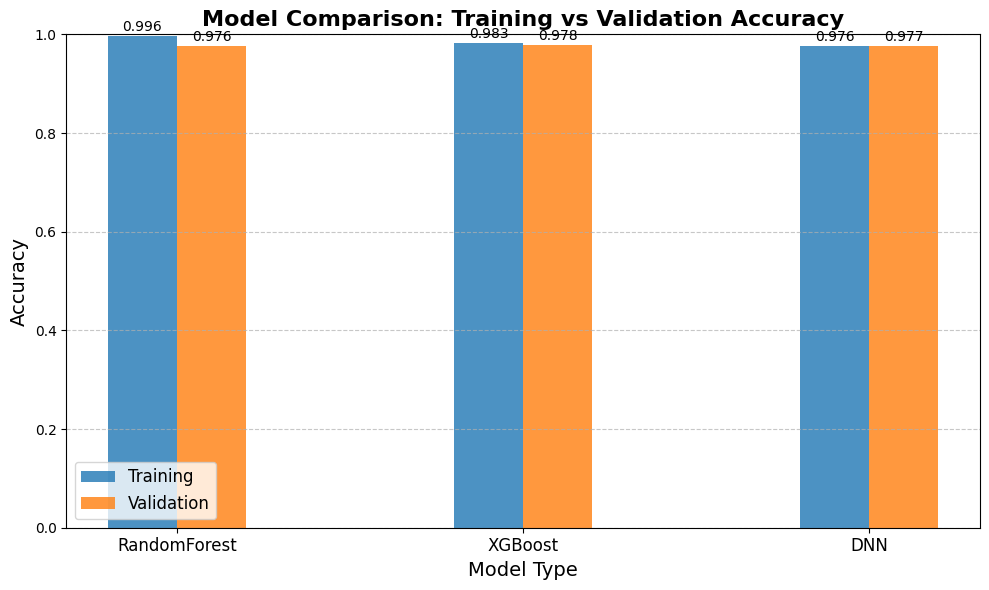
\includegraphics[width=\textwidth]{figures/2_top_model_cross_val_comparison.png}
        \caption{Comparison of top models with K-Fold Cross Validation}
    \end{subfigure}
    \begin{subfigure}[b]{0.7\textwidth}
        \centering
        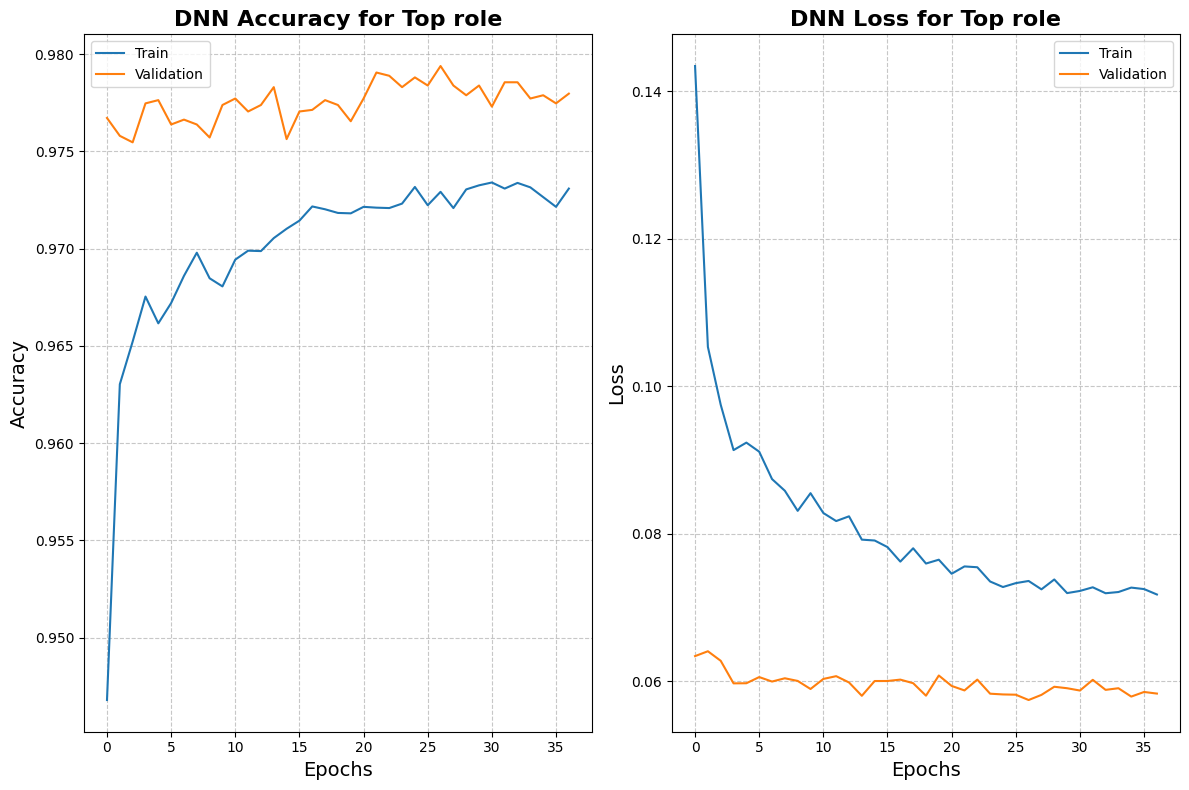
\includegraphics[width=\textwidth]{figures/2_top_model_cross_val_acc_loss.png}
        \caption{Top model accuracy and loss with K-Fold Cross Validation}
    \end{subfigure}
    \caption{K-Fold Cross Validation results}
    \label{fig:cross_val_comparison}
\end{figure}

The solution implemented was to train the NN model with different hyperparameters using \emph{for} loops and other models by using Cross Validation Grid Search so it only train 1 time on assured separated training/validation sets.
The Random Forest model was trained using range of values for the number of trees in the forest, the maximum depth of the trees, and the minimum number of samples required to split an internal node.
Note that it was also tested with \texttt{max\_depth=None} so nodes are expanded until all leaves are pure, and got better results but was increasing the training time a lot.
The XGBoost model was trained using different values of the number of boosting rounds, max depth, and learning rate.
The Neural Network was trained using different values of neurons in hidden layers, dropout values, and learning rates.
Every hidden layer uses ReLU activation function and are applied batch normalization and dropout.
To make sure that the model is not overfitting, L2 regularization of 0.1 was used on each hidden layer and, in fact, really do have made better results.

The metric used to evaluate the models was the accuracy on the validation set.
If a model has a higher accuracy, it keeps that model as the best current model and repeat the operation until finding the best overall model.

The results for each game role are shown in \appendixname~\ref{sec:top_model_training} for top, \appendixname~\ref{sec:jungle_model_training} for jungle, \appendixname~\ref{sec:mid_model_training} for mid, \appendixname~\ref{sec:bot_model_training} for bot, and \appendixname~\ref{sec:support_model_training} for support.
Results shows good accuracies for training and validation troughout all roles and NN accuracy/loss rapidly converges to them.
But I would still suspect that there still seems to be something wrong with the validation set as the accuracies are pretty high for not highly optimized models.
All of the roles except Mid role find best accuracies with the XGBoost model.
Mid got better results with the Neural Network model.
However, based on the results, they are all very close to each other and the differences are not significant.
Other parameters, features and ML concepts could be used like proper cross validation or PCA analysis for better features to see which one is really the best.

The final model is then used to predict the outcome of a game and the probability of winning or loosing on the test set.
The test set was created by splitting the dataset into 75\% training, 15\% validation, and 10\% test sets.
Surprisingly, the test set accuracy is close to the traning and validation accuracies.
This should not be the case, so there is still something that had been done wring in the training process or the dataset splitting.

\clearpage
\appendix
\section{Histogram representation of key features}\label{sec:features_histogram}
\begin{figure}[!ht]
    \centering
    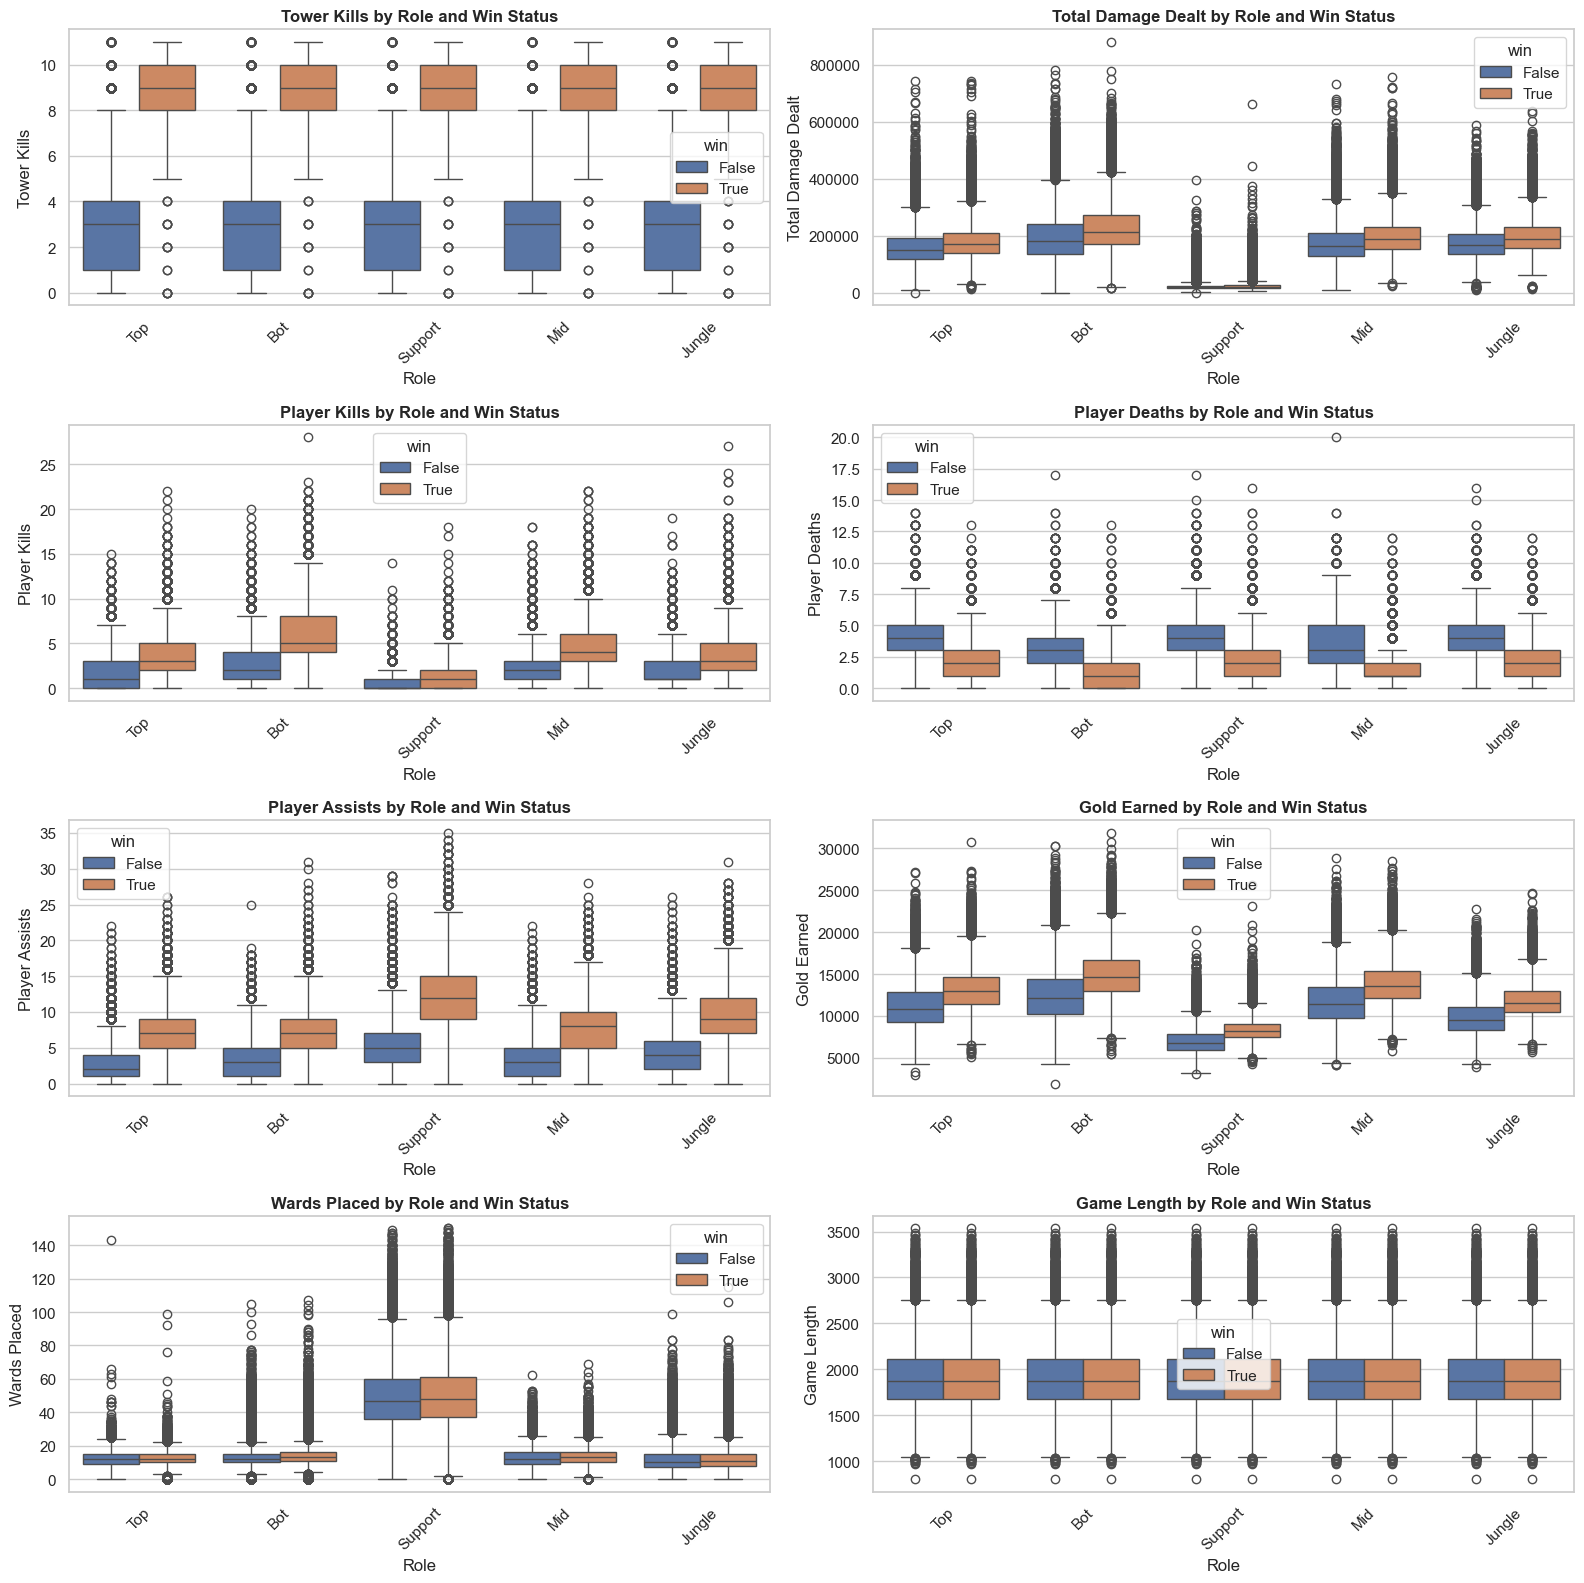
\includegraphics[width=0.9\textwidth]{figures/0_visualization_features_histogram_by_role.png}
\end{figure}

\clearpage
\section{Histogram representation of new features}\label{sec:new_features_histogram}
\begin{figure}[!ht]
    \centering
    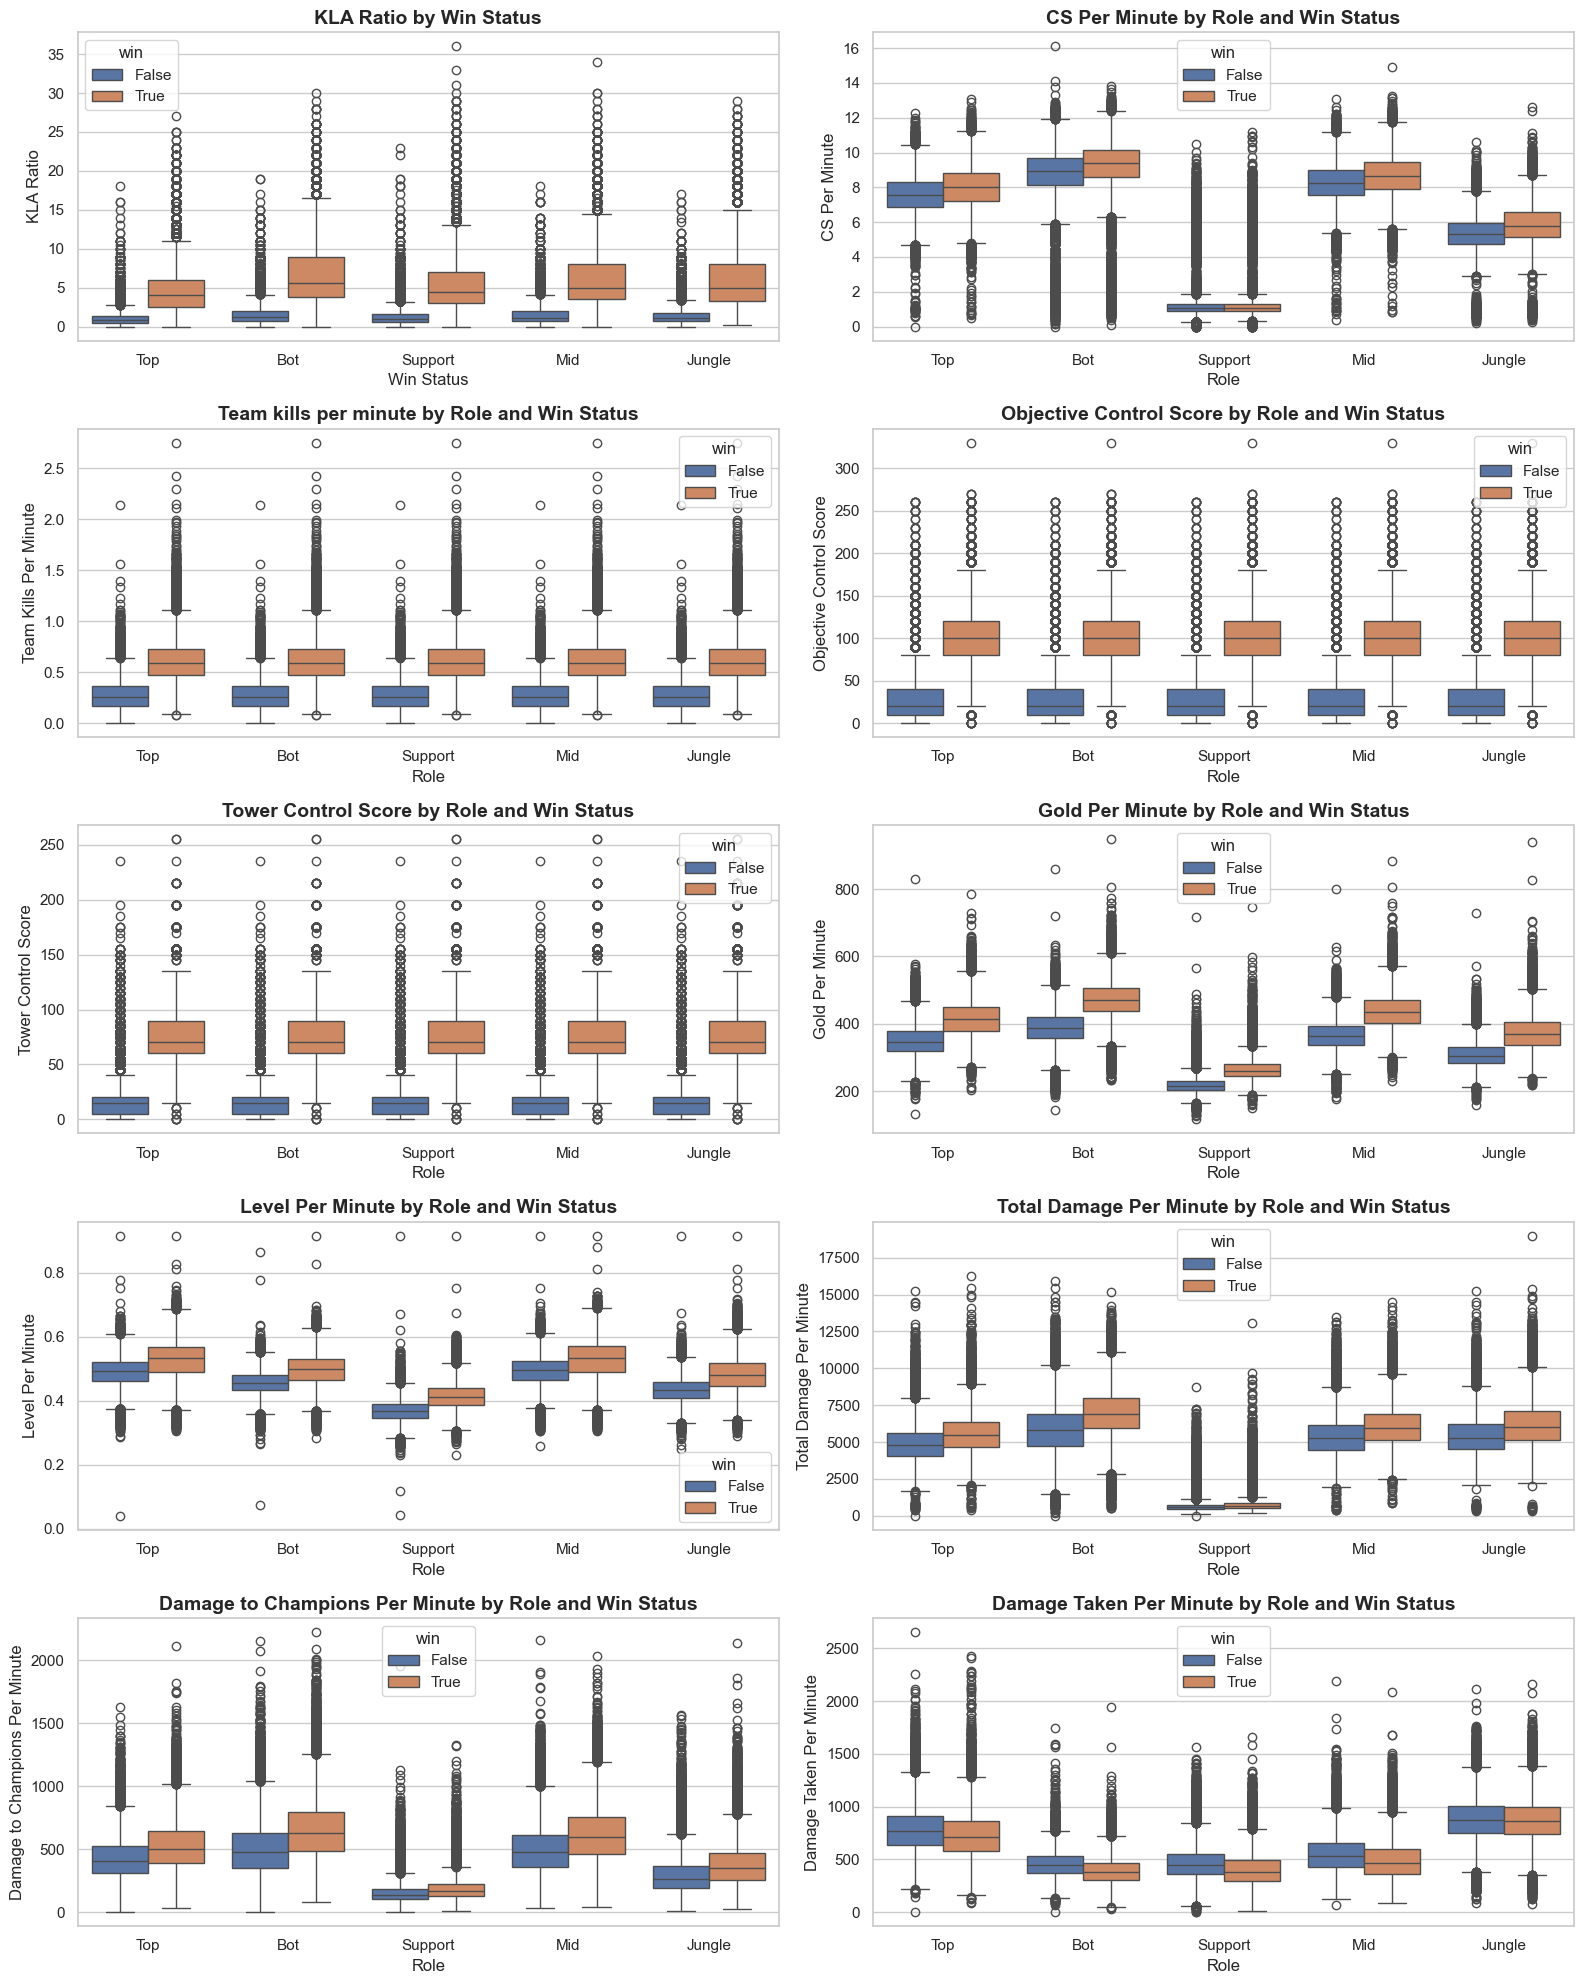
\includegraphics[width=0.9\textwidth]{figures/0_visualization_new_features_histogram_by_role.png}
\end{figure}

\clearpage
\section{Top model training and validation}\label{sec:top_model_training}
\begin{figure}[!ht]
    \centering
    \begin{subfigure}[b]{0.8\textwidth}
        \centering
        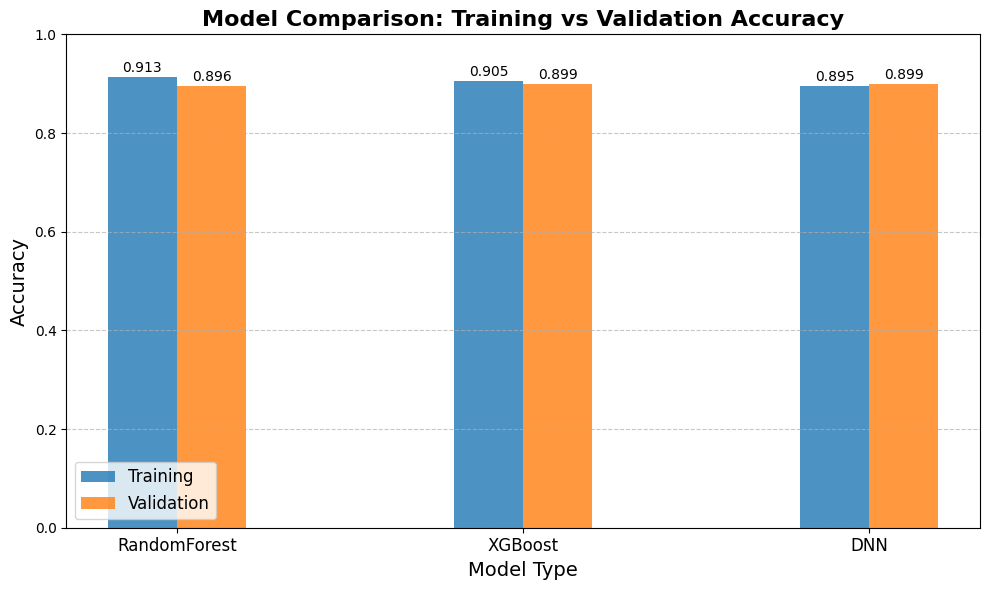
\includegraphics[width=\textwidth]{figures/2_top_model_comparison.png}
        \caption{Comparison of top models}
    \end{subfigure}
    \begin{subfigure}[b]{0.8\textwidth}
        \centering
        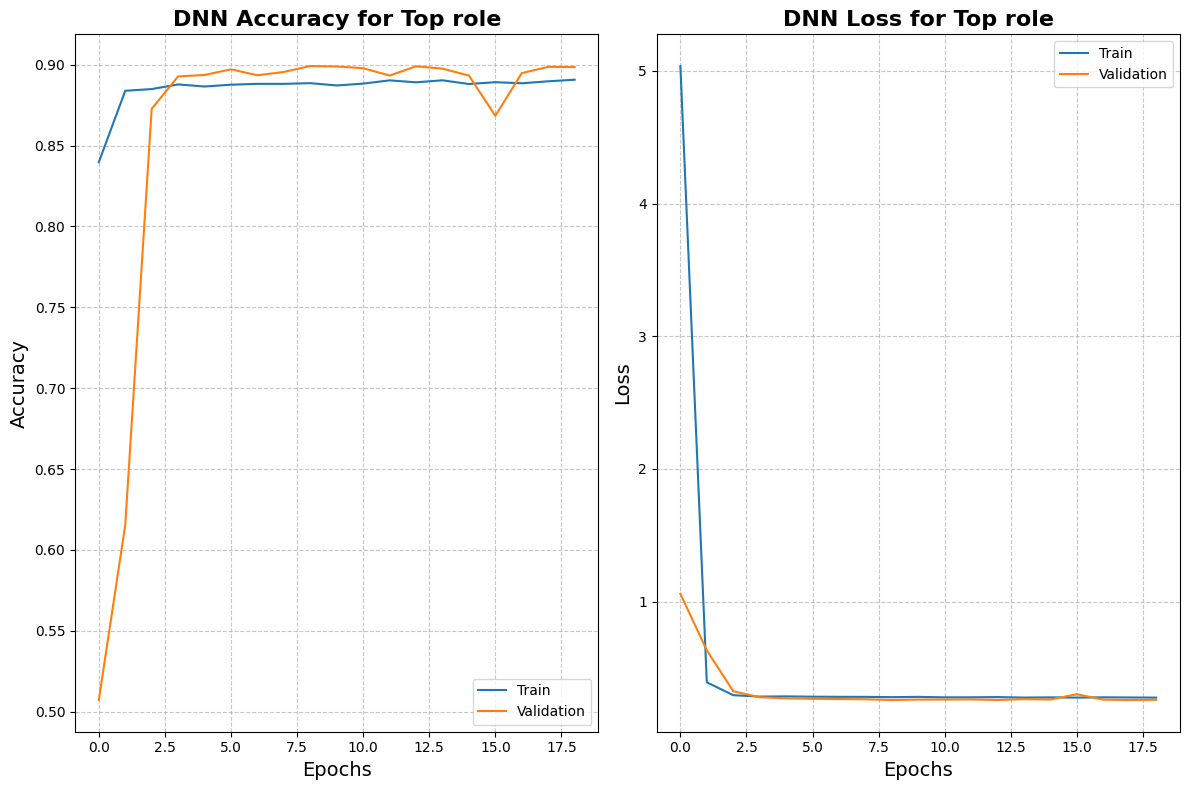
\includegraphics[width=\textwidth]{figures/2_top_model_acc_loss.png}
        \caption{Top model accuracy and loss}
    \end{subfigure}
\end{figure}

\clearpage
\section{Jungle model training and validation}\label{sec:jungle_model_training}
\begin{figure}[!ht]
    \centering
    \begin{subfigure}[b]{0.8\textwidth}
        \centering
        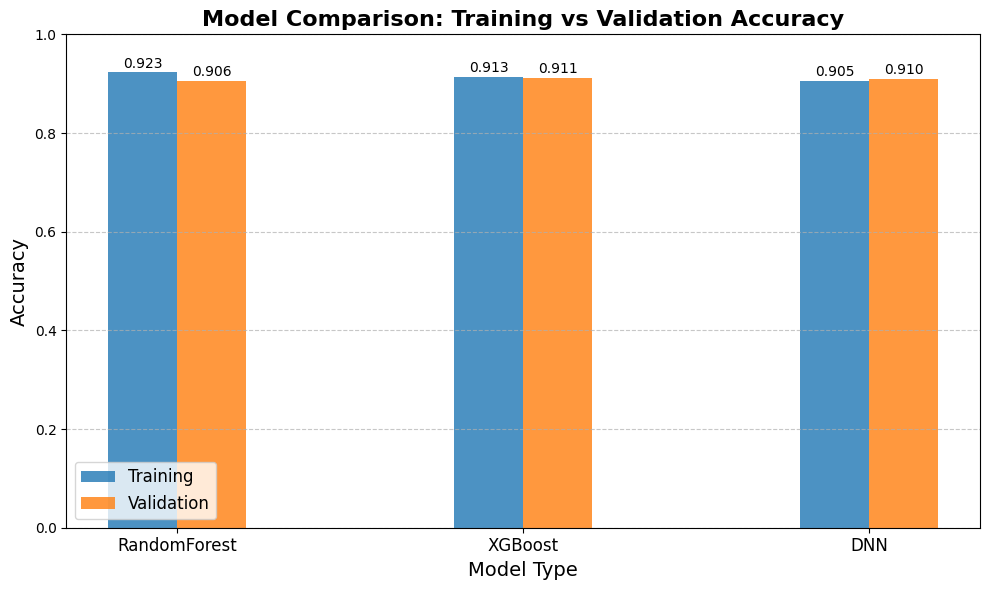
\includegraphics[width=\textwidth]{figures/2_jungle_model_comparison.png}
        \caption{Comparison of jungle models}
    \end{subfigure}
    \begin{subfigure}[b]{0.8\textwidth}
        \centering
        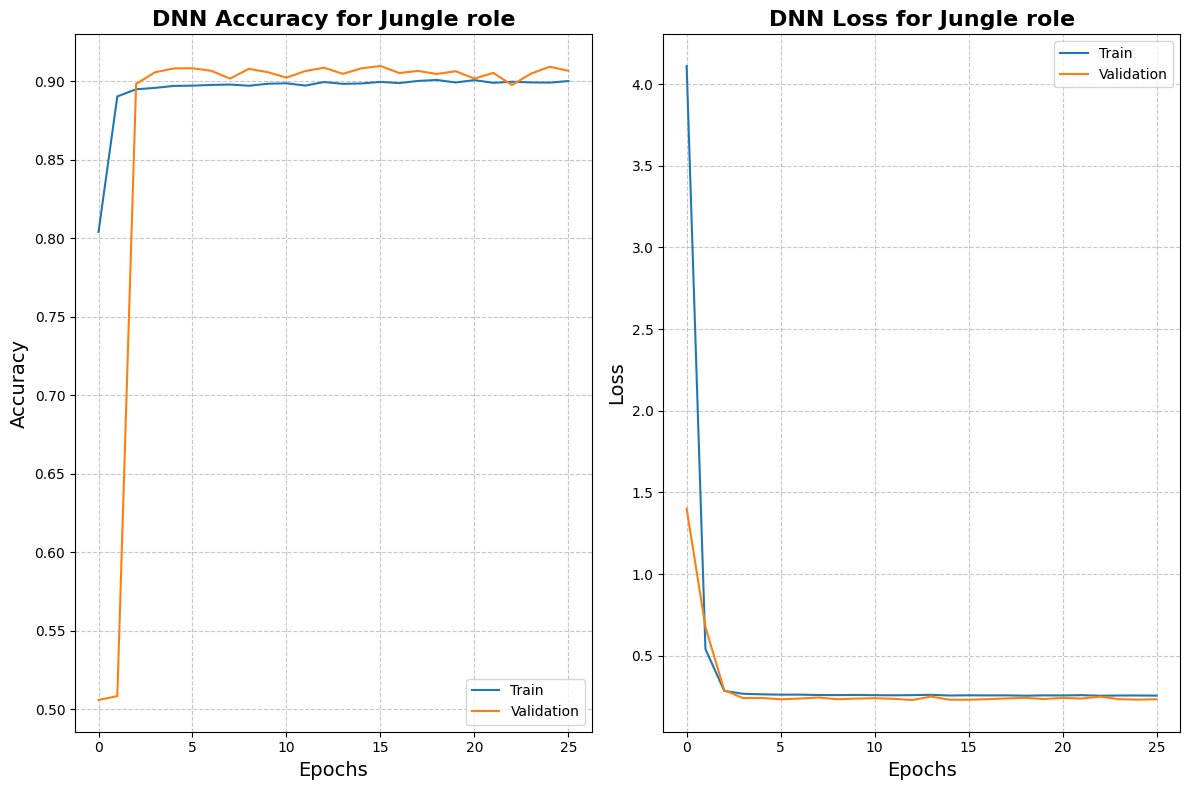
\includegraphics[width=\textwidth]{figures/2_jungle_model_acc_loss.png}
        \caption{Jungle model accuracy and loss}
    \end{subfigure}
\end{figure}

\clearpage
\section{Mid model training and validation}\label{sec:mid_model_training}
\begin{figure}[!ht]
    \centering
    \begin{subfigure}[b]{0.8\textwidth}
        \centering
        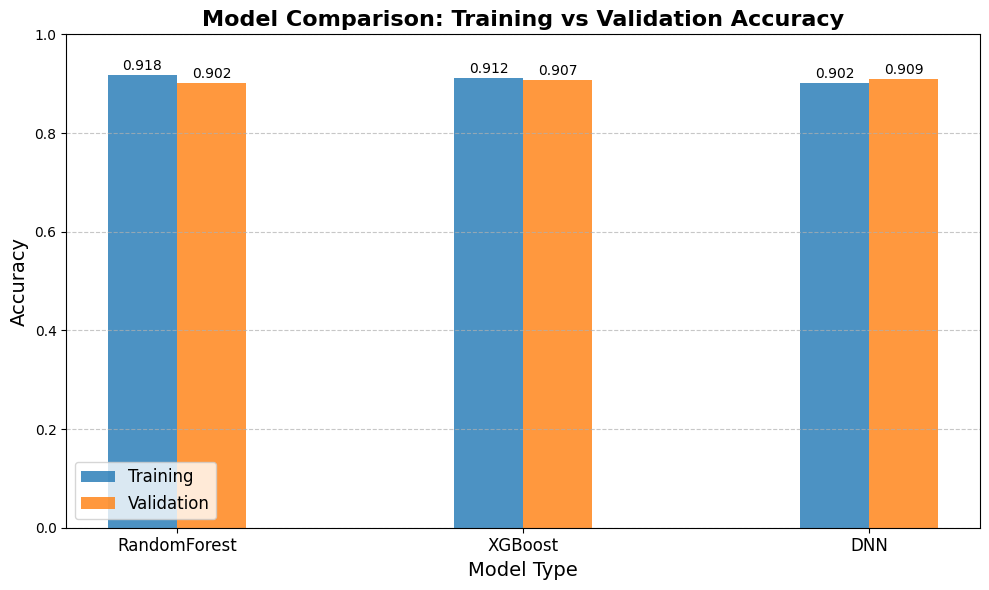
\includegraphics[width=\textwidth]{figures/2_mid_model_comparison.png}
        \caption{Comparison of mid models}
    \end{subfigure}
    \begin{subfigure}[b]{0.8\textwidth}
        \centering
        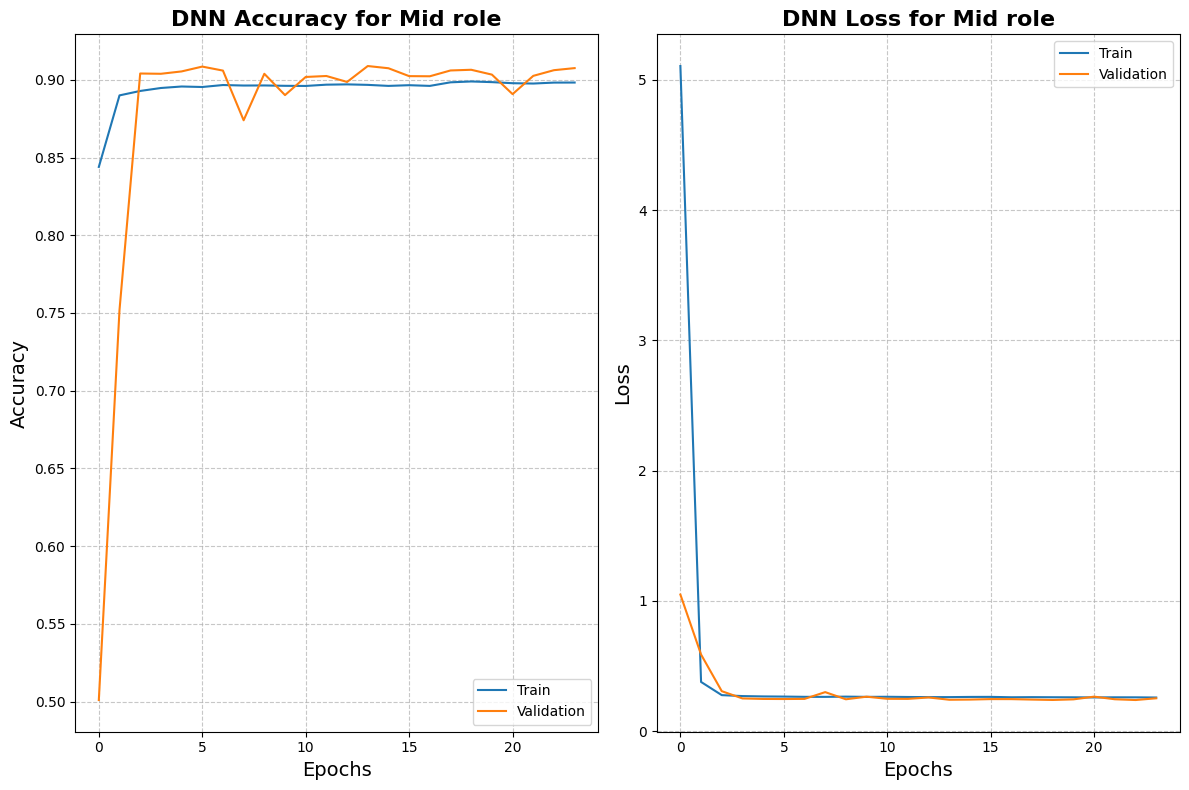
\includegraphics[width=\textwidth]{figures/2_mid_model_acc_loss.png}
        \caption{Mid model accuracy and loss}
    \end{subfigure}
\end{figure}

\clearpage
\section{Bot model training and validation}\label{sec:bot_model_training}
\begin{figure}[!ht]
    \centering
    \begin{subfigure}[b]{0.8\textwidth}
        \centering
        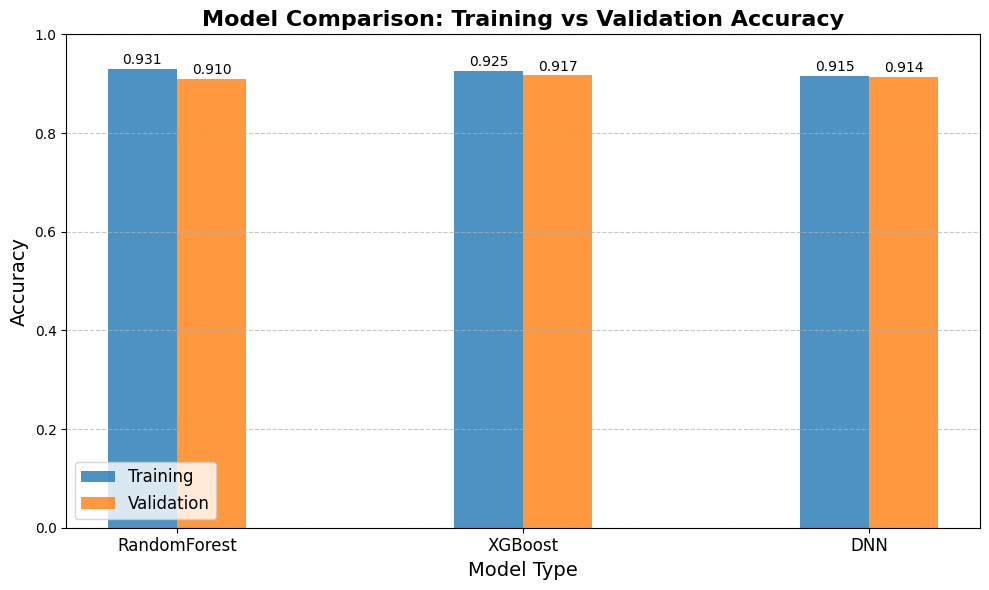
\includegraphics[width=\textwidth]{figures/2_bot_model_comparison.png}
        \caption{Comparison of bot models}
    \end{subfigure}
    \begin{subfigure}[b]{0.8\textwidth}
        \centering
        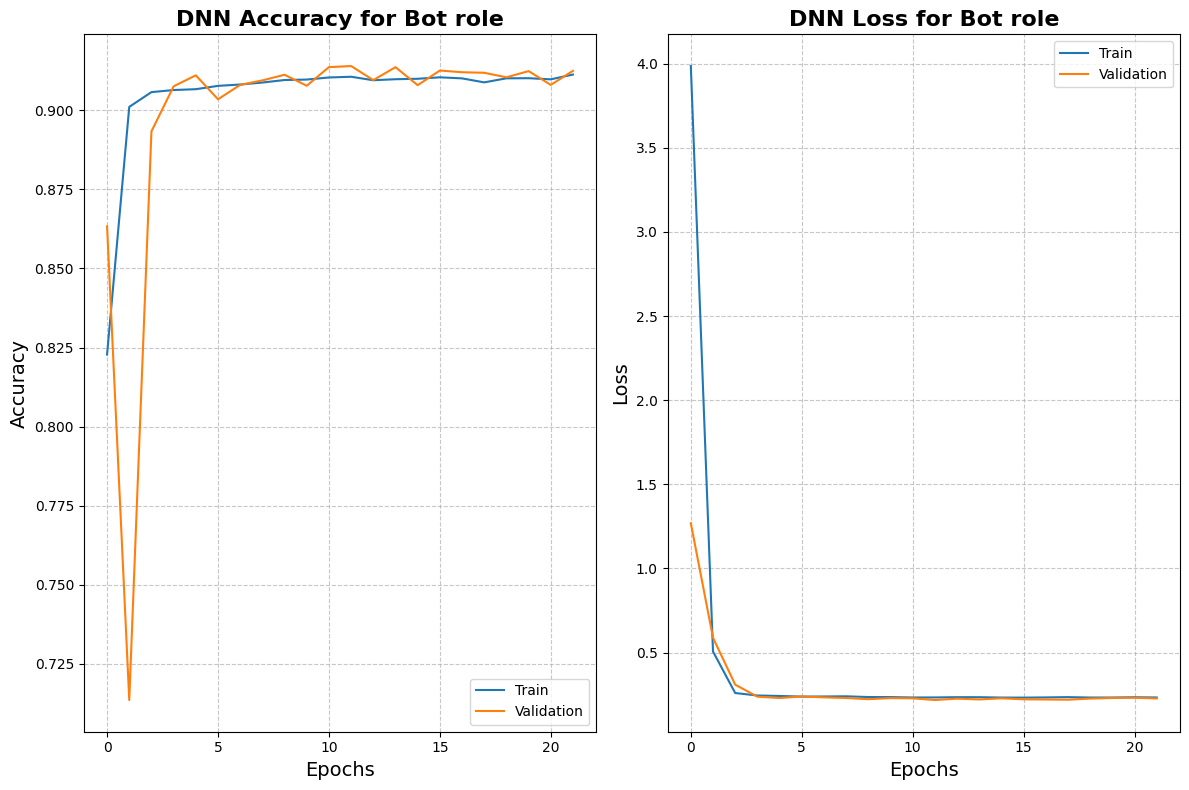
\includegraphics[width=\textwidth]{figures/2_bot_model_acc_loss.png}
        \caption{Bot model accuracy and loss}
    \end{subfigure}
\end{figure}

\clearpage
\section{Support model training and validation}\label{sec:support_model_training}
\begin{figure}[!ht]
    \centering
    \begin{subfigure}[b]{0.8\textwidth}
        \centering
        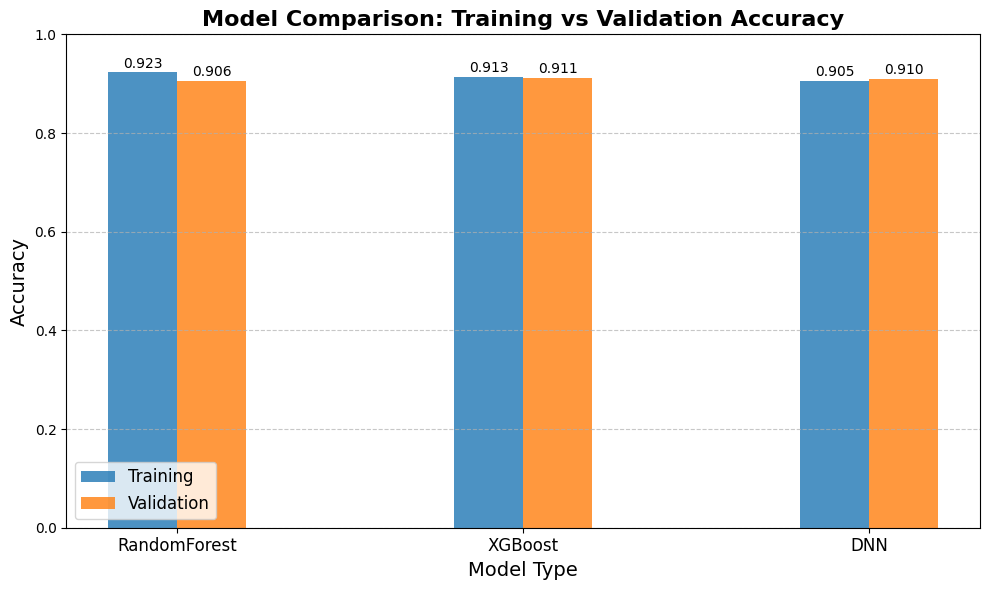
\includegraphics[width=\textwidth]{figures/2_support_model_comparison.png}
        \caption{Comparison of support models}
    \end{subfigure}
    \begin{subfigure}[b]{0.8\textwidth}
        \centering
        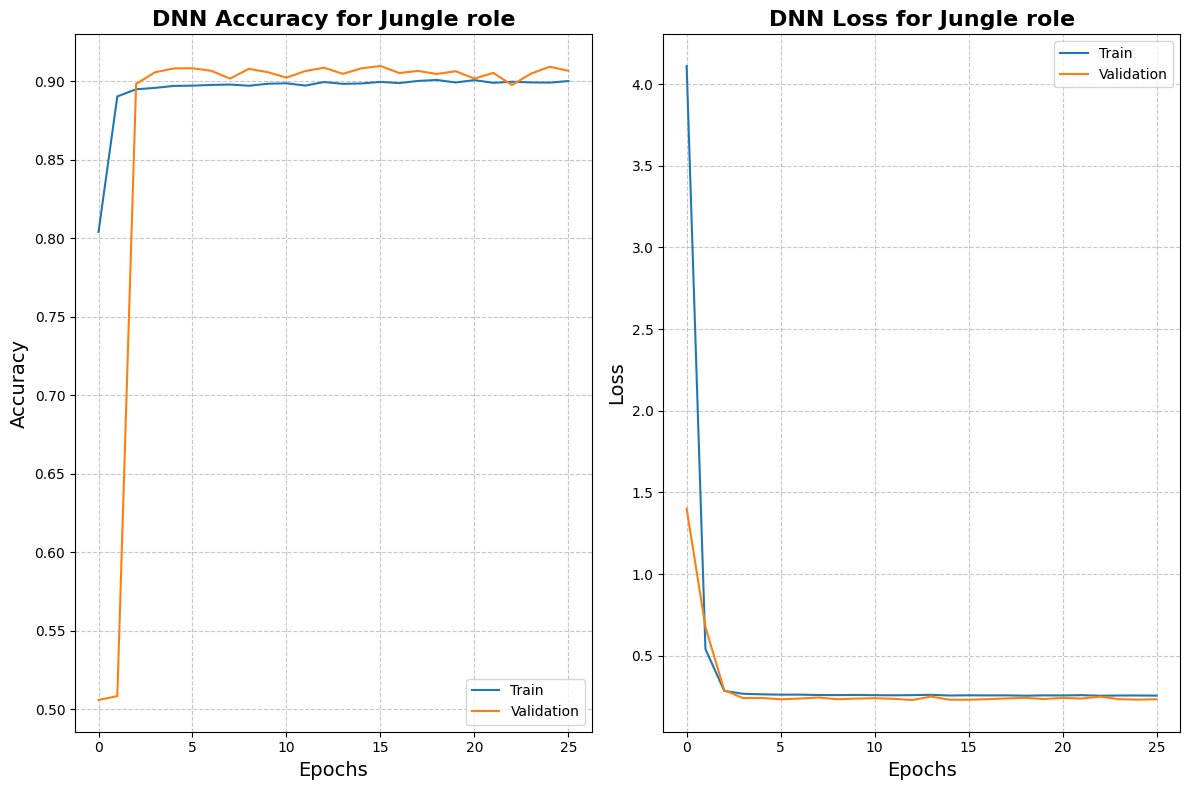
\includegraphics[width=\textwidth]{figures/2_support_model_acc_loss.png}
        \caption{Support model accuracy and loss}
    \end{subfigure}
\end{figure}

\end{document}